\chapter{Earth's surface water for the last 30 years - Aqua~Monitor}
\label{ch6}

\begin{abstract}
Has the world become wetter or drier? Can we see global trends in the changes of coastlines, and are these trends also apparent where we live?  Is the total surface water storage on land growing or shrinking at global and local scales?   This chapter presents results of the global surface water change study using data from all Landsat missions (2PB). All calculations were performed using Google Earth Engine infrastructure and the algorithm discussed in the previous chapter. The new tool, Aqua Monitor, illustrates how emerging cloud platforms for large satellite data analysis, are rapidly removing the thresholds to the use of planetary-scale data. The main finding of the Aqua Monitor show that the largest contributors to the transition between water and land include Aral Sea (water to land) and Tibetan Plateau (land to water). 

\begin{center}
	\begin{tikzpicture}[every node/.style={inner sep=0,outer sep=0}]
	\node[draw=none,shade,blur shadow={shadow blur steps=5}] {
		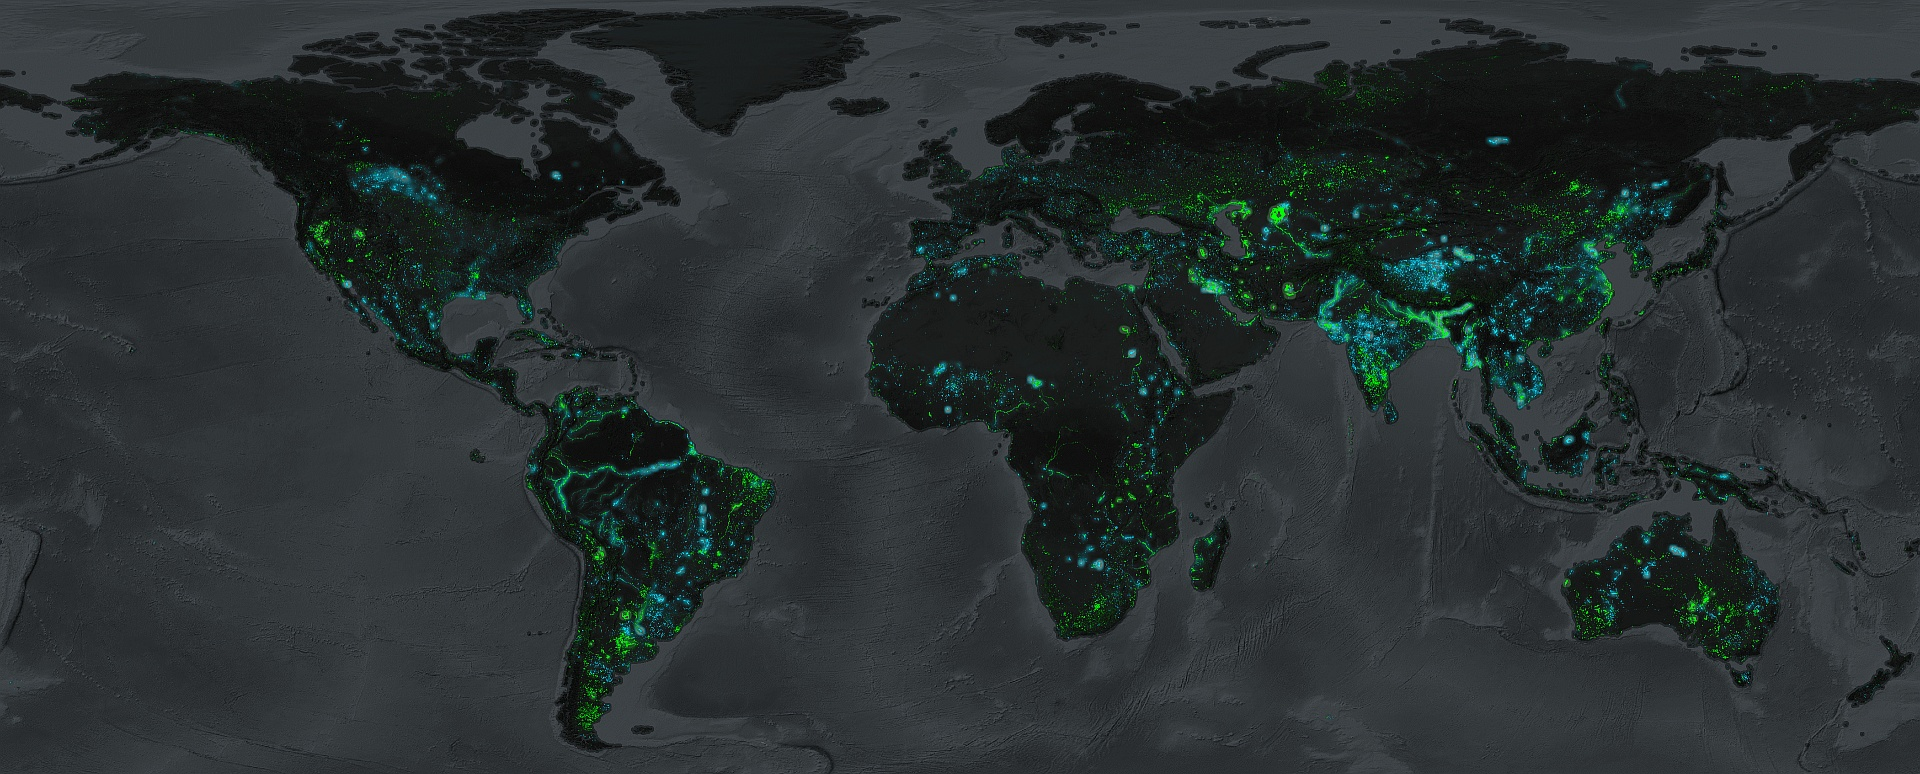
\includegraphics[width=0.7\textwidth]{01.8-aqua-monitor/figures/change-4k-small}
	};	
	\end{tikzpicture}
\end{center}

\textbf{Keywords:} global surface water changes, climate changes, land reclamation, erosion, accretion.

\end{abstract}

%% Start the actual chapter on a new page.
\newpage

\subsection{Introduction}
\dropcap{C}{hanges} from land to water and vice versa are extremely relevant as witnessed by many recent news items: rapid retreat of Tibetan Plateau glaciers observed during the last decades \citet{chen2016changes}; the impoundment of the Three Gorges Dam in China is causing massive inundations, forcing about 1.3 million people to resettle \citet{Jackson2000}; new islands along the coast of Dubai are created to provide new secluded areas for leisure and residence for the wealthy; and finally; the Mississippi Delta is losing thousands of hectares of land per year due to soil subsidence and lack of sediments \citet{Giosan2014}, further aggravated by sea-level rise; president of Kiribati declared that his people would need to move to new grounds to prevent them from dying from the effects of sea-level rise on the atoll \citet{Weiss2015}; 

The causality of appearing or disappearing water surfaces may strongly depend on the case‑specific context. Although atolls, such as Kiribati, are under severe threat, the exact effects of sea-level rise on coastal erosion, globally, may strongly depend on biophysical interactions as well, particularly in coastal marshes \citet{Storlazzi2015}, as atolls may increase accretion rates as sea-level rise progresses \citet{Kirwan2016}. The impoundment of the Three Gorges Dam has resulted in a reduction in sediment concentrations in the downstream Yangtze River of about 70\%. Unexpectedly, this reduction has not led to a retreat of the downstream submerged Yangtze River Delta so far \citet{Dai2014}, contrasting what happens in the Mississippi Delta.

These examples demonstrate that conversions - and the stories and reasons behind them - can vary widely and are often the result of compounding causes. Therefore, general conclusions cannot be drawn from a limited sample of case studies. Instead, planetary-scale monitoring is needed to understand (and disentangle) the causes of detected changes and their attribution to natural variability, climate change or man-made change. 

\section{Method to estimate Earth's long-term surface water changes}
To obtain changes in water and land occurrence, a method described in the Chapter \ref{ch4} is applied. The resulting algorithm was also implemented as an open-source website, called Deltares Aqua Monitor. Aqua Monitor prepares cloud-free average reflectance composite images for multiple years using all satellite images from all NASA Landsat missions and estimates surface water changes on-the-fly. The Deltares Aqua Monitor typically uses a 2-year period to obtain a sufficiently large number of images. However, to quantify long-term surface changes which have occurred during the last 30 years, we have extended this period to a longer baseline. The comparison was performed using two intervals: 1985-2005 and 2013-2016. The much longer first interval was required to ensure we have sufficiently large sample to compute statistics, as the number of images before 1999 is significantly larger when compared to recent years.

The Aqua Monitor establishes water-land and land-water occurrence on-the-fly by estimating the MNDWI spectral index values and performing trend analysis for these MNDWI values over both user-selected periods. For the analysis in this paper, these selected periods were 1985-2005 and 2013-2016 as mentioned above. To decrease noise for the high latitudes, all Landsat images acquired during night time are excluded. Additionally, we apply a topographic mask based on Height Above the Nearest Drainage3 (HAND) to decrease the noise in the hilly areas, occurring due to mismatches between sun elevation and azimuth parameters in both periods. All pixels representing mountain hills (HAND > 150m) are excluded, as described in \cite{donchyts2016imdp}. The final estimates of the surface area (land to water and water to land) were obtained by including pixels where large slope of the linear regression was observed.  

\section{Earth's surface water changes at 30m spatial resolution}

Because the spatial scale of many surface water changes is small, we have upscaled the final results (30m to 300m) in a form of two global images: \begin{enumerate*}[label=(\emph{\alph*})]
	\item surface water changes with transition water to land (green)
	\item surface water changes with transition land to water (blue)
\end{enumerate*}.

To produce the final global image and the Figure \ref{fig:am-heatmap}, both global images were mosaicked with an alpha channel, to ensure pixels where both change take place remain visible.

\begin{figure}
	\begin{adjustbox}{addcode={\begin{minipage}{\width}}{\caption{
						Heat map of global surface water and land changes. Blue lighting shows where land was converted into water over the period 1985-2015, Green lighting shows where water was converted into land over the same period. The intensity of the colors highlights the spatial magnitude of the change.
			}\label{fig:am-heatmap}\end{minipage}},rotate=90,center}
		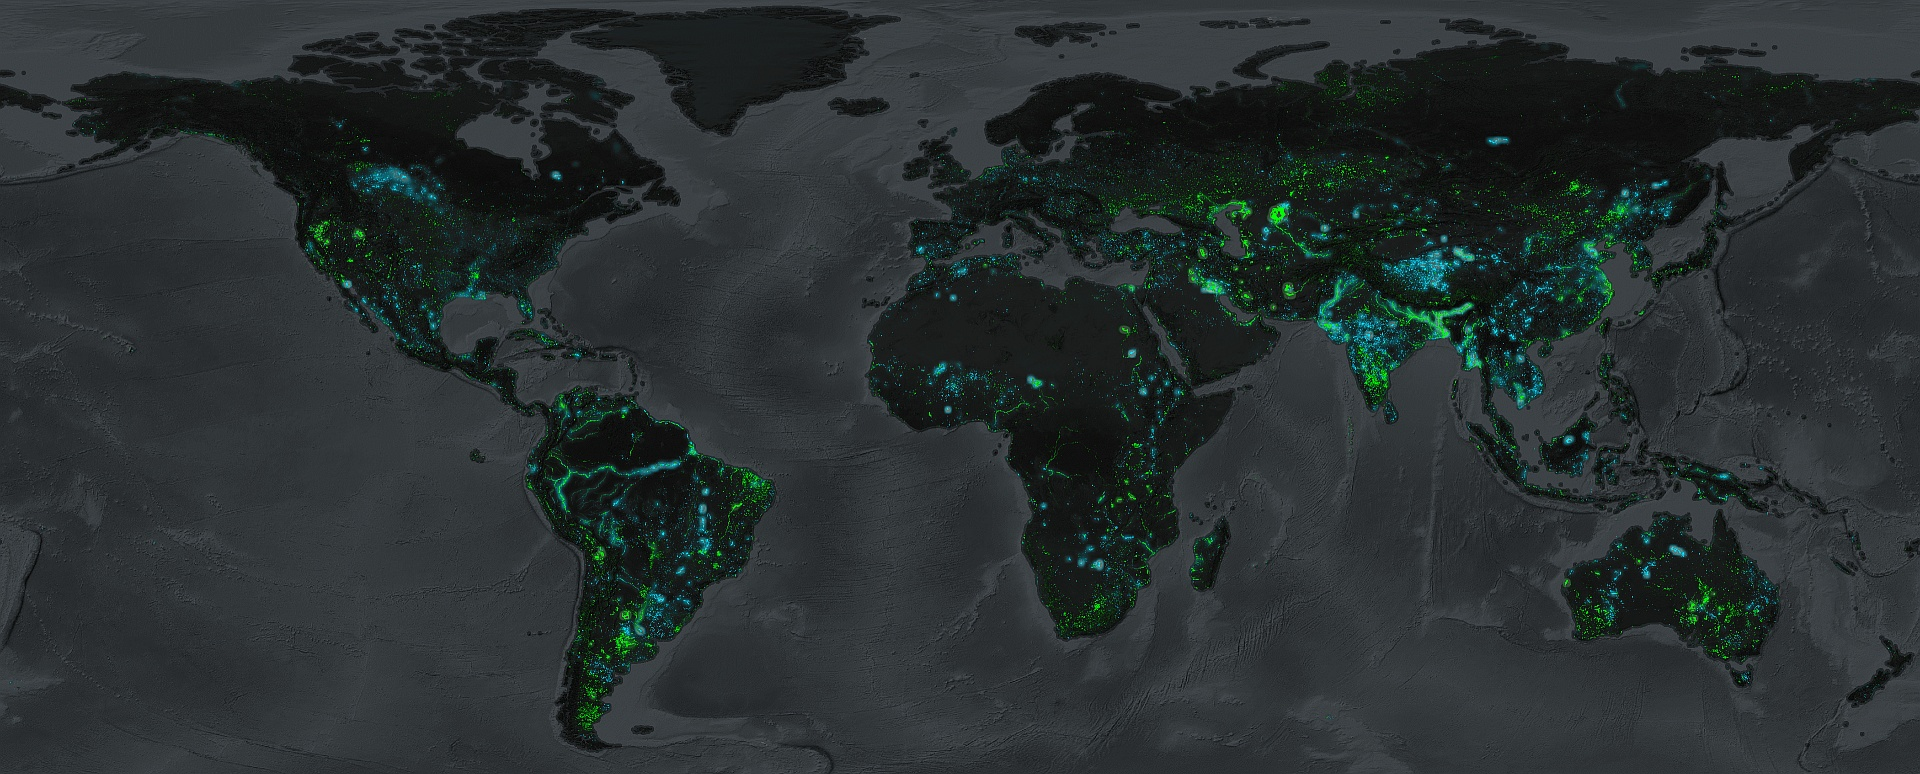
\includegraphics[width=1.0\textheight]{01.8-aqua-monitor/figures/change-4k-small}
	\end{adjustbox}
\end{figure}

\begin{figure}
	\begin{adjustbox}{addcode={\begin{minipage}{\width}}{\caption{
						Largest surface water and land changes from 1985 until 2015 grouped by drainage basins. Left: changes from land to water in blue. Right: changes from water to land in green.
			}\label{fig:am-drainage-basins}\end{minipage}},rotate=90,center}
		\includegraphics[width=0.9\textheight]{01.8-aqua-monitor/figures/Figure2}
	\end{adjustbox}
\end{figure}

The Deltares Aqua Monitor (\url{http://aqua-monitor.deltares.nl}) is the first global scale tool that shows at 30-m resolution where water is converted to land and vice versa. With assistance from Google Earth Engine, it analyses satellite imagery from multiple Landsat missions, which observed Earth for more than three decades on the fly. The Aqua Monitor provides a much needed \citet{Garcia2016}, fully planetary-scale view on changes in land and water occurrence. Documented and undocumented changes due to man-made interventions, natural variability and climate change are revealed. It is possible to look at any area of interest and use the outcomes for scientific advances at planetary-scale, review large-scale statistics on land and water conversion, or open a discussion with stakeholders in a given area on the basis of unbiased information on water and land occurrence and change.

\section{Surface water change examples}

This chapter demonstrates the planetary-scale ability of the Aqua Monitor by showing some significant and contrasting water–land conversions. It provides a perspective of what these abilities - which are now available to any researcher or stakeholder - mean for climate research. First, the planetary-scale changes in the occurrence of water and land are shown. It can be seen that globally, between 1985 and 2015, an area of about 173,000 $km^2$ — about the size of Washington State — has been converted to land, and an area of 115,000 $km^2$ has been converted into water. An overview of the largest changes found globally, aggregated per drainage basin \ref{fig:am-drainage-basins} identifies the \textbf{Tibetan Plateau} and the \textbf{Amazon River} as the areas with the largest area conversion to water. The \textbf{Aral Sea} is the standout for conversion to land. As changes in surface water only affect people at a regional and local scale, we show some contrasting cases for different areas \ref{fig:am-examples} and describe these below.

\begin{figure}[H]
	\centering
	\includegraphics[width=1\textwidth]{01.8-aqua-monitor/figures/Figure3}
	\caption{Examples of surface water changes between 1987 and 2015, detected using Aqua Monitor. Blue: conversion from land to water. Green: conversion from water to land}
	\label{fig:am-examples}
\end{figure}

\subsection{Known and unknown (Myanmar vs North Korea)}
Although many countries report on their dam construction, information in more remote or isolated areas is lacking. In Myanmar, the Global Reservoir and Dams database \citet{Lehner2011} shows an increase in water surface between 1985 and 2010 of about 400 $km^2$. Using the Aqua Monitor, we have counted the appearance of 1,180 $km^2$ of new water surface in this region over the same period (Figure \hyperref[fig:am-examples]{\ref{fig:am-examples}a}). The previously unmapped damming of the Rimjin River in North Korea, close to the border with South Korea, resulted in a storage surface of 12.4 $km^2$ (Figure \hyperref[fig:am-examples]{\ref{fig:am-examples}b}). This is, in fact, the Hwanggang Dam, at the time of writing mapped 35 km eastward. The dam was the topic of an international dispute between South and North Korea after the 2009 flash flood that killed six fisherman \citet{SangHun2009}.

\subsection{Luxury versus needs (Dubai vs Sinapore)}
The largest coastal water–land change is the construction of the Palm Island and adjacent islands along the coast of Dubai 80 $km^2$; (Figure \hyperref[fig:am-examples]{\ref{fig:am-examples}c}). Many countries have shaped and extended their coastlines by land reclamation. The motives to reclaim land are highly diverse. In Dubai, the main motivation was to increase the coast length, providing more room for recreation \citet{Davidson2009}. In contrast, reclamations in Singapore (76 $km^2$; Figure \hyperref[fig:am-examples]{\ref{fig:am-examples}d}) are necessary to support its economic growth \url{http://www.mnd.gov.sg/landuseplan}).

\subsection{Nature versus Man-made (Ganges-Brahmaputra Delta vs Taji Najer Lake)}
Results of the Aqua Monitor only show compound impacts of natural and human change or variability. It is often hard to tell what the causes are for a change without looking at the details of the local water
and sediment budget. Although changes in meanders in the Brahmaputra River Delta are clearly natural (Figure \hyperref[fig:am-examples]{\ref{fig:am-examples}e}), the Mondrianlike shapes formed near Taiji Nai’er lakes in China, are clearly man-made (Figure \hyperref[fig:am-examples]{\ref{fig:am-examples}f)}.

\subsection{Disruptive versus gradual (Aral Lake vs Lake Mead)}
An example of disruptive change can be found at the Aral Sea, once the fourth-largest lake in the world. Since the 1960s, Soviet engineers diverted the rivers away from this endorheic lake to irrigate cotton and wheat agriculture \citet{Glantz1999}. The lake has almost entirely dried up, losing about 27,650 $km^2$ of surface water (Figure \hyperref[fig:am-examples]{\ref{fig:am-examples}g}). The positive impacts of a recent restoration program \citet{Micklin2016} in the northern part can be observed as well. A slower drying lake can be found near Las Vegas at Lake Mead, the largest freshwater supply in the United States. It lost 222 $km^2$ over the same period (Figure \hyperref[fig:am-examples]{\ref{fig:am-examples}h}). The 10\% probability scenario that the lake would have already dried out by 2013 \citet{Barnett2008} did not come true, but the lack of inflow from the Colorado River will cause the lake to gradually disappear.

\section{Near-shore coastal surface water changes}
One of the questions which can be answered by remote sensing is how much surface water changes took places along the global coastline. This can be important to detect effects such as sea level raise and other changes caused by natural processes or anthropogenic factors. Some of examples of the natural processes causing the largest coastline changes are migration of mudbanks along the \href{http://aqua-monitor.appspot.com/?from=2000&to=2016&view=5.37464731850053,-52.96134948730469,11z}{East-North part of South America}, causing erosion and accretion of the coastline and mangrove areas up to 3km in width; changes along the coastline surrounding the \href{http://aqua-monitor.appspot.com/?mode=dynamic&from=2000&to=2016&view=29.161696898682372,-89.24575805664062,11z}{mouth of the Mississippi River}, though here many of these processes are also reported to be caused by man-made changes, such as construction of levees, causing reduction of deposits of fresh water and silt from the river; erosion and accretion of the \href{http://aqua-monitor.appspot.com/?from=2000&to=2016&view=22.47760292118218,90.76316833496092,9z}{Brahmaputra River Delta}, causing appearance of 20m long islands and erosion of large areas - this is probably the area where the largest natural changes take place along the coastline. 

At the same time, we can conclude from the results of our study, that many man-made changes along the coast have resulted in a reclamation of the large areas of the ocean. When not considering the Aral Sea, the major contributor to the man-man changes is China, where about 6000 $km^2$ of new land has been claimed from the sea. Land reclamation occurs practically along the whole \href{http://aqua-monitor.appspot.com/?from=2000&to=2016&view=27.965842094147863,120.95462799072264,11z}{Chinese coastline}, resulting in the areas up to 5km wide claimed from the seas.

Even though this would be a very interesting study to perform on its own, we have tried to roughly estimate these near-shore changes. One of the main challenges we have faced when performing this analysis is to select a baseline coastline. To our experience, the accuracy of all existing and freely available vector and raster datasets defining coastline is insufficient for this kind of study, mainly because the coastline is dynamic in many locations. Therefore, a multi-step approach is required to firstly estimate the baseline coastline for a given period and then, to compute relative long-term surface water changes from this baseline. To simplify the analysis, we have used 40km buffer around OpenStreetMap coastline, followed by aggregation of these changes for every country. The resulting surface areas for both accretion and erosion are reported in the Figure \ref{fig:am-coasline}.

\begin{figure}
	\centering
	\includegraphics[width=1\textwidth]{01.8-aqua-monitor/figures/Figure4}
	\caption{Largest land-water changes within 40km distance around the coastline from 1985 until 2015. Light colors indicate country-scale changes, while bright colours show the actual location of the changes. Left: changes from land to water. Right: changes from water to land.}
	\label{fig:am-coasline}
\end{figure}

\section{Conslusions and Discussion}
Big satellite data analytics at anyone’s fingertips, may have strong implications on monitoring capacities and associated actions. At a very local scale, a civilian can now assess without any expert assistance, if coastal erosion threatens their house. At a regional scale, a downstream riparian state can monitor from year to year, if upstream neighbours are establishing new impoundments. Finally, at a global scale, agencies such as the United Nations International Strategy for Disaster Reduction can monitor the appearance of new, possibly flood hazard reducing, reservoir storage capacity.

Implications for climate research follow from the fact that the available time series are long enough to cover a climatologically relevant period. The period of 30 years allows distinction between noise of (multi)
annual variations, such as the lake surface area of Lake Nasser, and long-term trends in land and water distribution, such as the vanishing of the Aral Sea. Feeding changes in land and water surfaces into regional climate models will lead to better representation of circulation patterns, as well as local climate, in particular in the vicinity of large wetlands \citet{Mohamed2005}. Another example is the attribution to sea-level rise or other drivers of coastal erosion in soft sediment coastal areas \citet{Barros2015}. Drivers such as sea-level rise, sediment delivery and subsidence, and the biophysical properties of the coastline, can cause highly nonlinear erosion and accretion. Quantifying the contribution of these drivers would benefit tremendously from information on multiscale patterns of erosion and accretion from low global) to very high (local) resolution. The climate community is presented with the capacity to take into account these new planetary-scale observation abilities.
